\section{Messungen}
Die entwickelte Platine

\begin{figure}[h!]
	\centering
	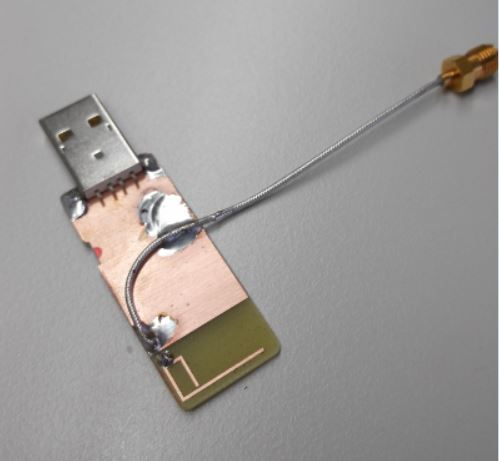
\includegraphics[width=0.5\textwidth]{../fig/plt/Platine.JPG}
	\caption{Die entwickelte Platine}
	\label{fig:Platine}
\end{figure}




\subsection{Messungen mit dem Netzwerkanalyzer}

Marke: Rhode$\&$Schwartz\\
Inventarnr.: 14006

\vspace*{3mm}

Vor dem Einsatz des Netzwerkanalyzers wurde dieser kalibiert.

\begin{figure}[h!]
	\centering
	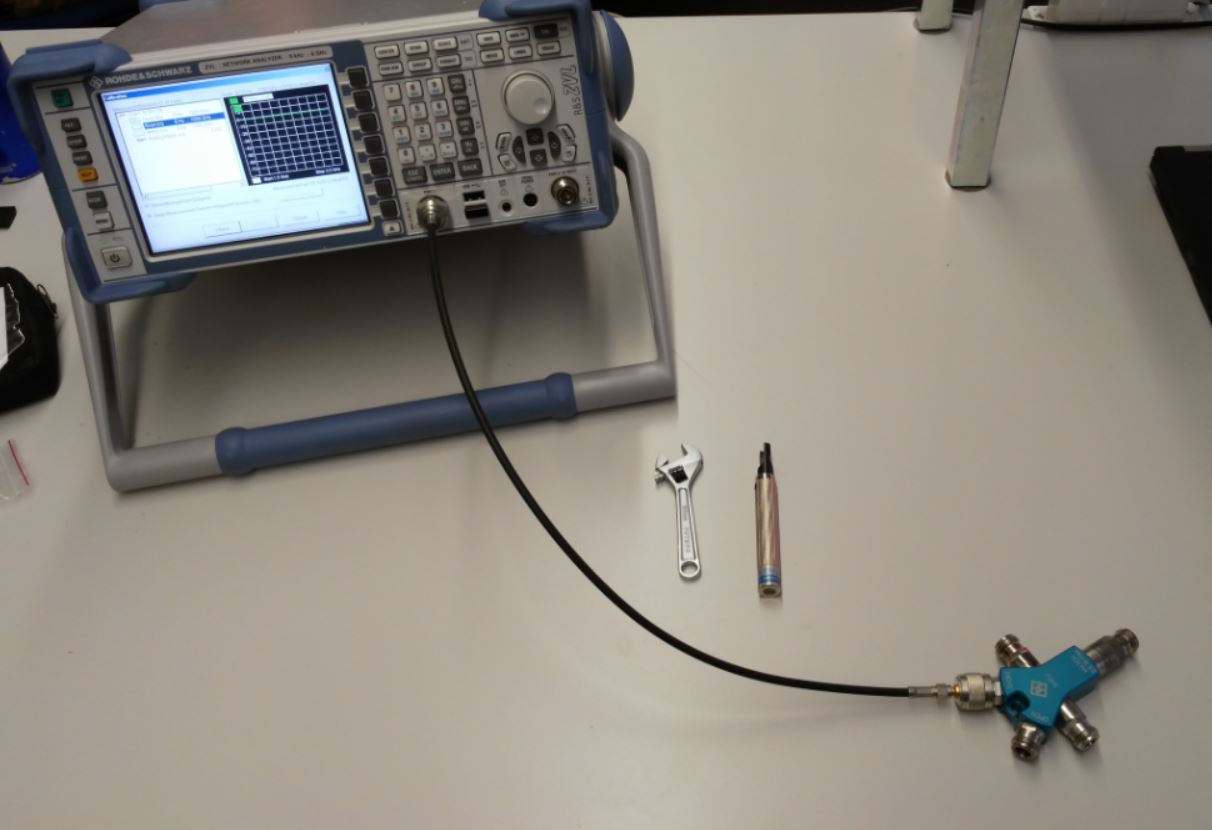
\includegraphics[width=0.8\textwidth]{../fig/plt/Calib.JPG}
	\caption{Kalibrierung des Netzwerkanalyzers}
	\label{fig:calib}
\end{figure}

Mit dem Netzwerkanalyzer wurden Messungen ohne und mit Gehäuse gemacht bei 2.4 GHz und 5 GHz. In diesem Bericht wird der Fokus  auf die Messung mit Gehäuse gelegt. Zum einen Überblick über das gesamte Frequenzspektrum zu vermitteln.
Abbildungen x zeigen einen Überblick über das gesamte Frequenzspektrum von 1.75 GHz bis 5.75 GHz.  Im Abschnitt x und Abschnitt y wird auf die Messungen bei den spezifischen Designfrequenzen eingegangen.

\begin{figure}[htbp]
	\begin{center}
		\begin{subfigure}[t]{0.49\textwidth}
			\begin{center}
				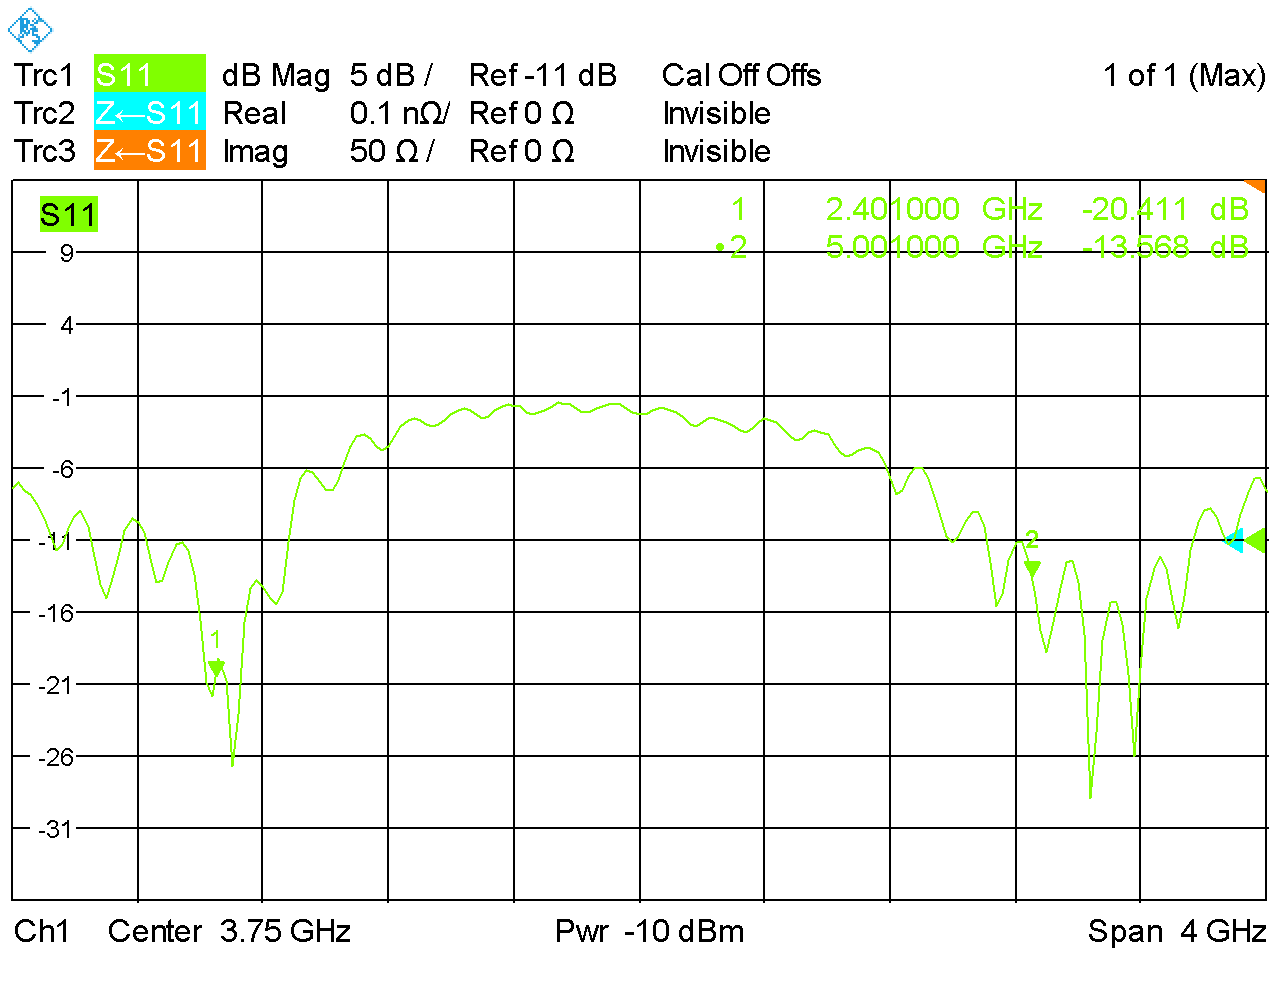
\includegraphics[width=1\textwidth]{../fig/plt/S11_WITH_FULL.PNG}
				\caption{Reflexionskoeffizient}
				\label{fig:S11_with_full}
			\end{center}
		\end{subfigure}
		\begin{subfigure}[t]{0.49\textwidth}
			\begin{center}
				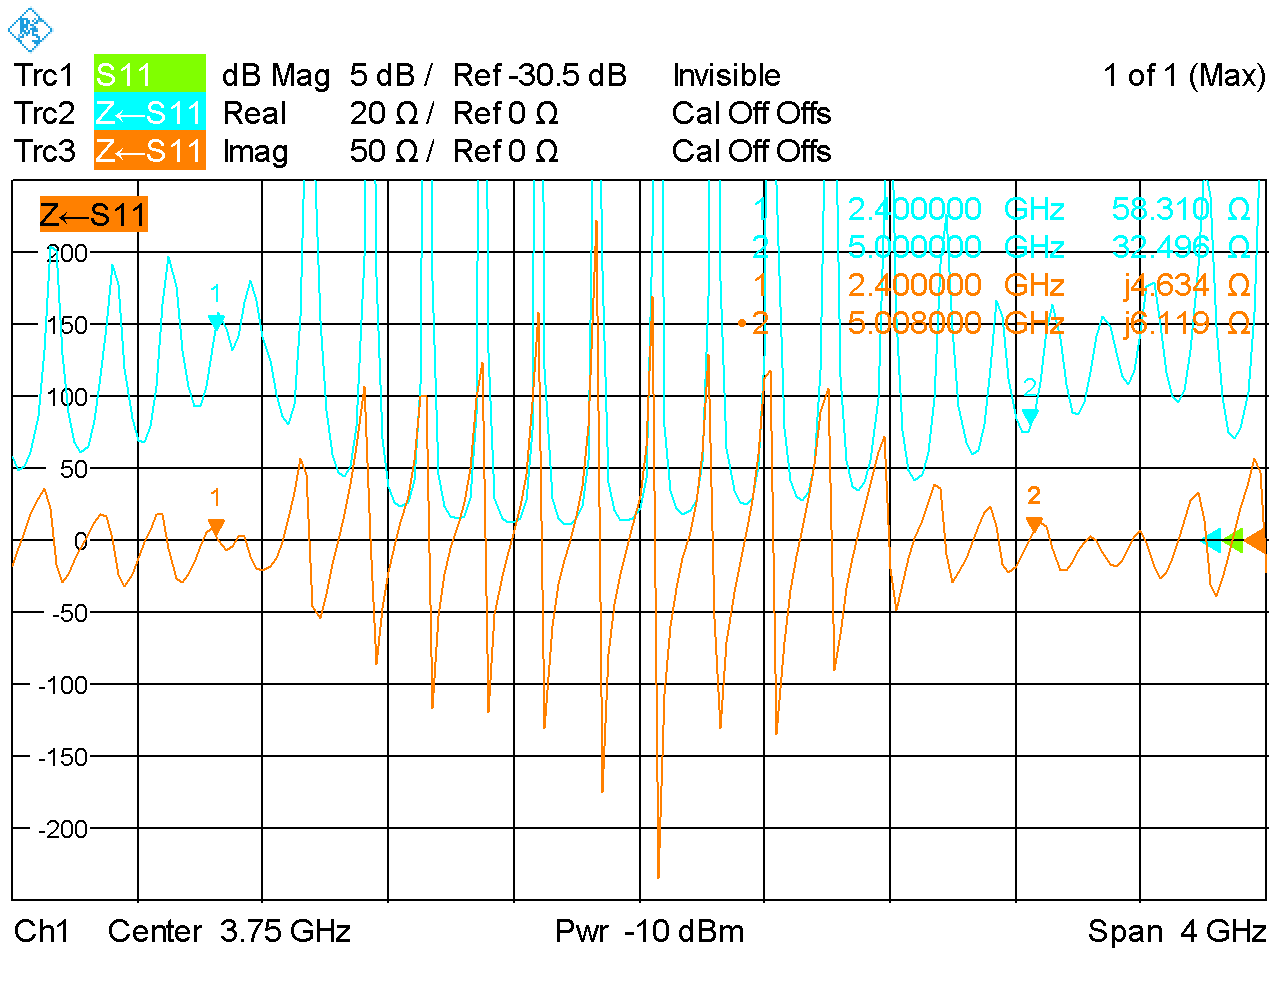
\includegraphics[width=1\textwidth]{../fig/plt/IMP_WITH_FULL.PNG}
				\caption{Impedanz}
				\label{fig:Imp_with_full}
			\end{center}
		\end{subfigure}
		\caption{Überblick über gesamtes Frequenzspektrum}
		\label{fig:full}
	\end{center}
\end{figure}


\subsubsection{Reflexionskoeffizient S11}

Bei 2.4 GHz zeigte sich ein äusserst ausgeprägter Reflexionskoeffizent kleiner als -50dB

\begin{figure}[htbp]
	\begin{center}
		\begin{subfigure}[t]{0.49\textwidth}
			\begin{center}
				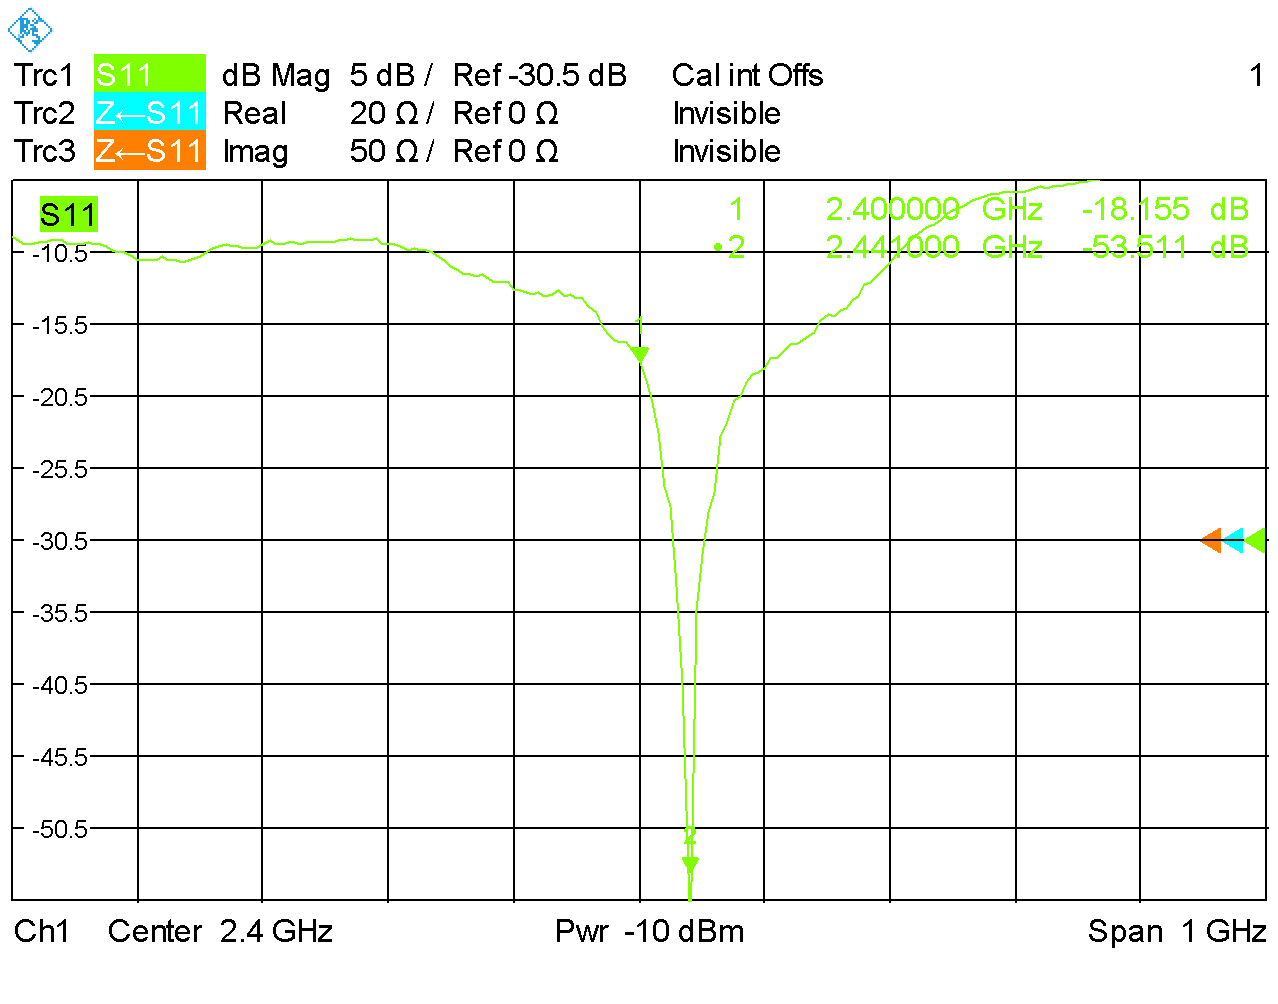
\includegraphics[width=1\textwidth]{../fig/plt/S11_WITH_2_4.PNG}
				\caption{bei 2.4 GHz}
				\label{fig:S11_with_full_2.4}
			\end{center}
		\end{subfigure}
		\begin{subfigure}[t]{0.49\textwidth}
			\begin{center}
				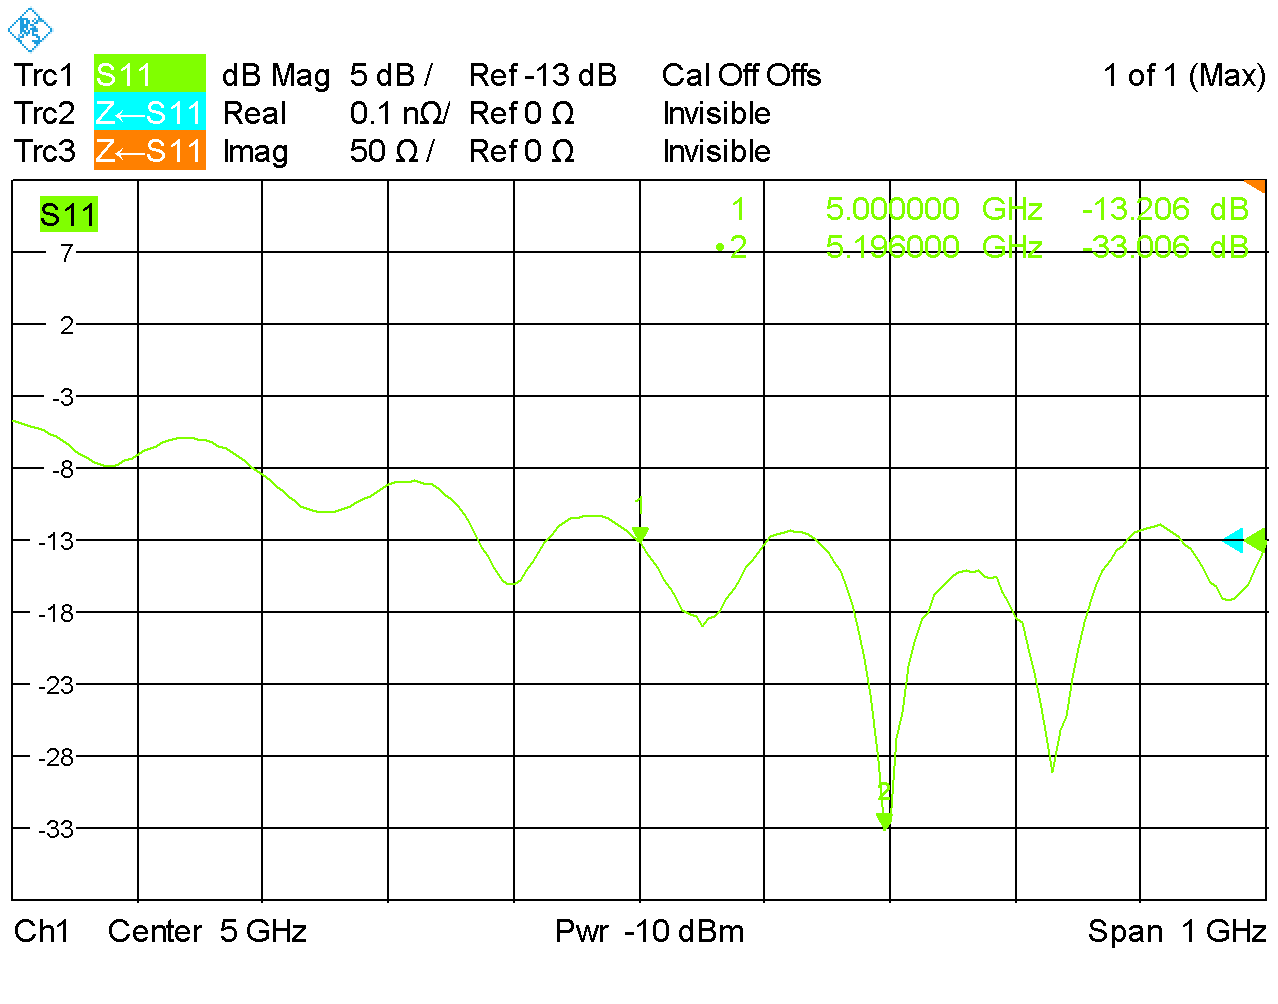
\includegraphics[width=1\textwidth]{../fig/plt/S11_WITH_5_0.PNG}
				\caption{bei 5.0 GHz}
				\label{fig:S11_with_full_5.0}
			\end{center}
		\end{subfigure}
		\caption{Reflexionskoeffizient S11}
		\label{fig:S11_each}
	\end{center}
\end{figure}

\subsubsection{Impedanz}

\begin{figure}[htbp]
	\begin{center}
		\begin{subfigure}[t]{0.49\textwidth}
			\begin{center}
				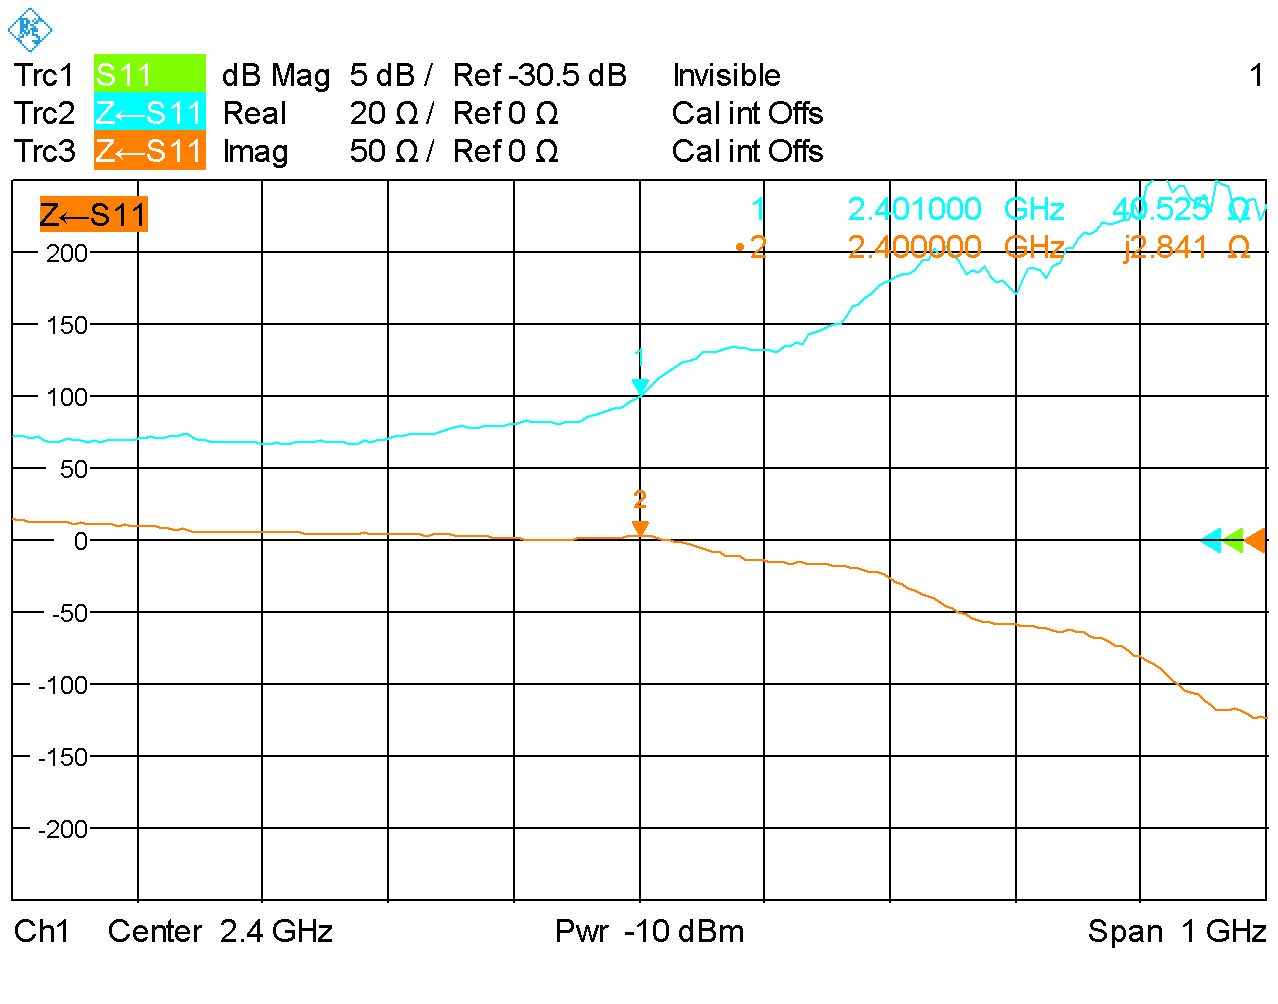
\includegraphics[width=1\textwidth]{../fig/plt/IMP_WITH_2_4.PNG}
				\caption{bei 2.4 GHz, !Achtung falsche Skala!}
				\label{fig:Imp_with_full_2.4}
			\end{center}
		\end{subfigure}
		\begin{subfigure}[t]{0.49\textwidth}
			\begin{center}
				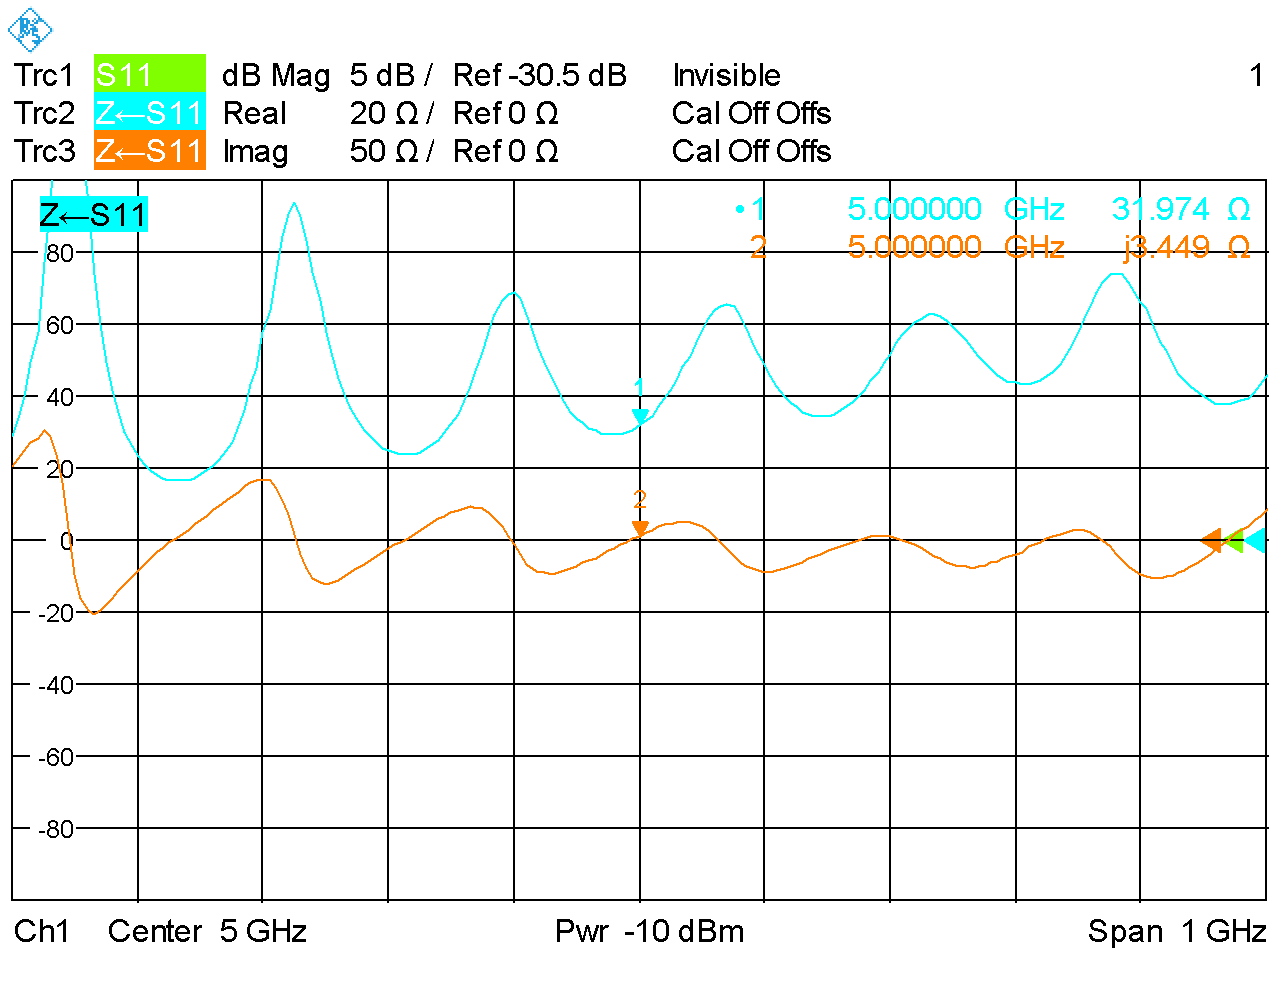
\includegraphics[width=1\textwidth]{../fig/plt/IMP_WITH_5_0.PNG}
				\caption{bei 5.0 GHz}
				\label{fig:Imp_with_full_5.0}
			\end{center}
		\end{subfigure}
		\caption{Impedanzen}
		\label{fig:Imp_each}
	\end{center}
\end{figure}

\newpage
\subsection{Messungen mit dem Starlab}

\begin{figure}[h!]
	\centering
	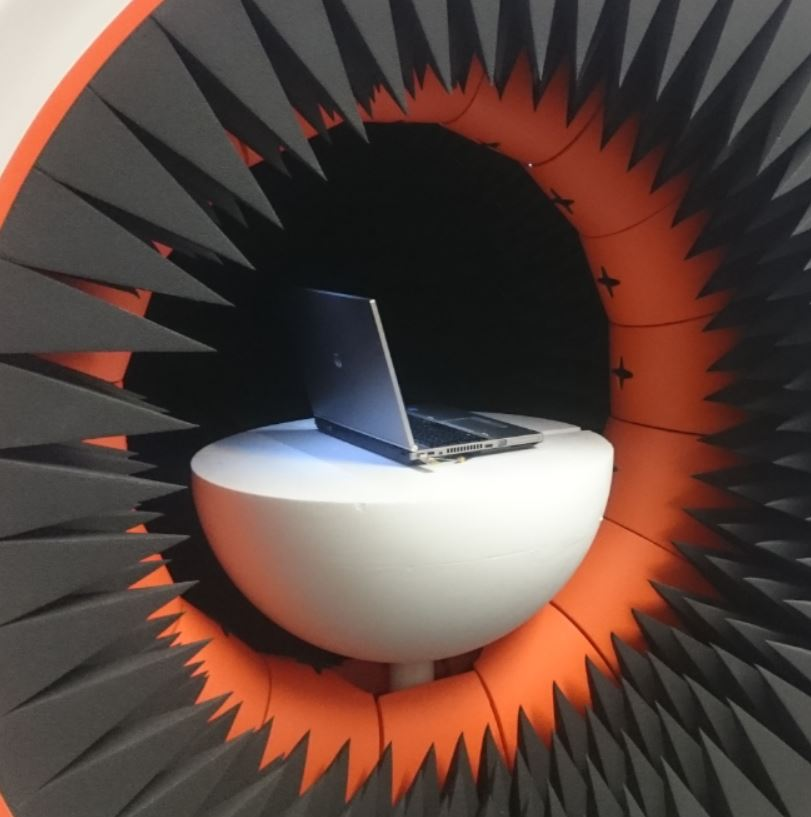
\includegraphics[width=0.6\textwidth]{../fig/plt/LaptopimStarLab.JPG}
	\caption{DUT eingesteckt am Laptop im LinearScanner}
	\label{fig:LaptopimStarlab}
\end{figure}
